\documentclass[tikz,border=12pt]{standalone}
\usepackage[T1]{fontenc}
\usepackage{tgheros}
\usepackage{sfmath}
\usepackage{amsmath}
\usepackage{fontawesome5}
\usepackage{tikz}
\usetikzlibrary{arrows.meta,positioning,shapes.geometric,fit,backgrounds,calc}
\usepackage{xcolor}

\renewcommand{\familydefault}{\sfdefault}

% Semantic Palette from visual-system.md
\definecolor{navy}{HTML}{1B2A4A}
\definecolor{navylight}{HTML}{E8EDF6}
\definecolor{teal}{HTML}{168F84}
\definecolor{teallight}{HTML}{E4F6F3}
\definecolor{amber}{HTML}{C98218}
\definecolor{amberlight}{HTML}{FFF3DC}
\definecolor{coral}{HTML}{BD4F2F}
\definecolor{corallight}{HTML}{FAE9E2}
\definecolor{violet}{HTML}{6550A8}
\definecolor{violetlight}{HTML}{F0ECFA}
\definecolor{slate}{HTML}{687386}
\definecolor{slatelight}{HTML}{F4F6F7}
\definecolor{cardborder}{HTML}{CBD5E1}

\begin{document}
\begin{tikzpicture}[
  font=\sffamily,
  >=Stealth,
  flowcard/.style={
    draw=cardborder,
    fill=white,
    rounded corners=5pt,
    line width=1.1pt,
    inner sep=8pt,
    minimum height=1.9in,
    align=center,
    text=navy
  },
  toxiccard/.style={
    draw=coral,
    fill=corallight,
    rounded corners=5pt,
    line width=1.2pt,
    inner sep=8pt,
    minimum height=1.9in,
    align=center,
    text=navy
  },
  safecard/.style={
    draw=teal,
    fill=teallight,
    rounded corners=5pt,
    line width=1.2pt,
    inner sep=8pt,
    minimum height=1.9in,
    align=center,
    text=navy
  },
  brancharrow/.style={
    ->,
    line width=1.1pt,
    draw=navy!80
  },
  coralarrow/.style={
    ->,
    line width=1.4pt,
    draw=coral
  },
  tealarrow/.style={
    ->,
    line width=1.4pt,
    draw=teal
  },
  badgelabel/.style={
    font=\sffamily\scriptsize\bfseries,
    fill=white,
    draw=cardborder,
    rounded corners=2pt,
    inner sep=2.5pt,
    align=center,
    text=navy
  }
]

  % Top Banner
  \node[draw=navy!30, fill=slatelight, rounded corners=4pt, line width=0.8pt, text width=7.6in, align=center, inner sep=6pt] (topbanner) {
    \textbf{\faIcon{sync-alt}\; POLICY ENDOGENEITY: NAIVE FLYWHEEL VS. GOVERNED EPISODE SLICING}\\[2pt]
    {\footnotesize Why raw human intervention logging destroys behavioral cloning policies, and how sliced lineages restore stability}
  };

  % =========================================================================
  % ROW 1: NAIVE UN-TAGGED FLYWHEEL (POISONOUS)
  % =========================================================================
  \node[toxiccard, text width=2.25in, below=0.45in of topbanner.south west, anchor=north west] (n_event) {
    \textbf{\color{coral}\faIcon{exclamation-circle}\; 1. Takeover Event}\\[2pt]
    {\scriptsize Robot heads toward obstacle; operator grabs joystick and steers sharp right.}\\[4pt]
    \rule{2.0in}{0.4pt}\\[4pt]
    \begin{minipage}{2.1in}
    \scriptsize
    $\bullet$ Pre-crash drift: $[s_{t-k}, a_{\text{drift}}]$\\
    $\bullet$ Human panic save: $[s_t, a_{\text{steer}}]$\\
    $\bullet$ Closed-loop endogeneity unmanaged
    \end{minipage}
  };

  \node[toxiccard, text width=2.25in, right=0.42in of n_event] (n_log) {
    \textbf{\color{coral}\faIcon{database}\; 2. Naive Logging}\\[2pt]
    {\scriptsize Single contiguous stream recorded without takeover boundary tag.}\\[4pt]
    \rule{2.0in}{0.4pt}\\[4pt]
    \begin{minipage}{2.1in}
    \scriptsize
    $\bullet$ Drift and save merged blindly\\
    $\bullet$ No demarcation of human input\\
    $\bullet$ Covariate shift enters dataset
    \end{minipage}
  };

  \node[toxiccard, text width=2.25in, right=0.42in of n_log] (n_train) {
    \textbf{\color{coral}\faIcon{skull-crossbones}\; 3. Policy Collapse}\\[2pt]
    {\scriptsize Retrained policy fits spurious causal link between obstacle proximity and turn.}\\[4pt]
    \rule{2.0in}{0.4pt}\\[4pt]
    \begin{minipage}{2.1in}
    \scriptsize
    $\bullet$ \textbf{Spurious Rule:} "Speed into pillars"\\
    $\bullet$ Multi-modal distribution blur\\
    $\bullet$ Catastrophic bench collision
    \end{minipage}
  };

  \draw[coralarrow] (n_event.east) -- (n_log.west);
  \draw[coralarrow] (n_log.east) -- (n_train.west);

  % Branch Divider Label
  \coordinate (mid_left) at ($(n_event.south west)+(0, -0.22in)$);
  \coordinate (mid_right) at ($(n_train.south east)+(0, -0.22in)$);
  \draw[dashed, line width=0.8pt, draw=slate!50] (mid_left) -- (mid_right);
  \node[fill=white, draw=slate!40, rounded corners=3pt, inner sep=3pt, font=\sffamily\scriptsize\bfseries, text=navy] 
    at ($(mid_left)!0.5!(mid_right)$) {\faIcon{shield-alt}\; THE GOVERNED DATA FILTER BOUNDARY};

  % =========================================================================
  % ROW 2: GOVERNED SLICED FLYWHEEL (SAFE & REPRODUCIBLE)
  % =========================================================================
  \node[safecard, text width=2.25in, below=0.42in of n_event.south west, anchor=north west] (g_event) {
    \textbf{\color{teal}\faIcon{tag}\; 1. Hardware Tagging}\\[2pt]
    {\scriptsize Real-time MCU detects takeover $\|\mathbf{u}_{\text{h}}\| > \delta_{\text{takeover}}$ and stamps PTP hardware clock.}\\[4pt]
    \rule{2.0in}{0.4pt}\\[4pt]
    \begin{minipage}{2.1in}
    \scriptsize
    $\bullet$ Takeover timestamp $t_{\text{takeover}}$\\
    $\bullet$ IEEE 1588 PTP sync ($\pm 1\,\mu\text{s}$)\\
    $\bullet$ Hardware telemetry lineage nonce
    \end{minipage}
  };

  \node[safecard, text width=2.25in, right=0.42in of g_event] (g_slice) {
    \textbf{\color{teal}\faIcon{cut}\; 2. Episode Slicing}\\[2pt]
    {\scriptsize Automated partition isolates pre-crash failure from corrective recovery.}\\[4pt]
    \rule{2.0in}{0.4pt}\\[4pt]
    \begin{minipage}{2.1in}
    \scriptsize
    $\bullet$ Discard window: $[-T_{\text{discard}}, 0] \to \mathcal{D}_{\text{fail}}$\\
    $\bullet$ Recovery demo: $[0, T_{\text{rec}}] \to \mathcal{D}_{\text{recov}}$\\
    $\bullet$ Nominal slice: $\mathcal{D}_{\text{nominal}}$ pristine
    \end{minipage}
  };

  \node[safecard, text width=2.25in, right=0.42in of g_slice] (g_lineage) {
    \textbf{\color{teal}\faIcon{fingerprint}\; 3. Governed Lineage}\\[2pt]
    {\scriptsize Cryptographic hash chain binds trained weights to audited dataset partition.}\\[4pt]
    \rule{2.0in}{0.4pt}\\[4pt]
    \begin{minipage}{2.1in}
    \scriptsize
    $\bullet$ $\text{SHA-256}(\mathcal{D}_{\text{clean}}) \leftrightarrow \text{SHA-256}(W)$\\
    $\bullet$ Shadow-mode replay evaluation gate\\
    $\bullet$ Stable autonomous release
    \end{minipage}
  };

  \draw[tealarrow] (g_event.east) -- (g_slice.west);
  \draw[tealarrow] (g_slice.east) -- (g_lineage.west);

  % Bottom Provenance Strip
  \node[draw=navy!30, fill=slatelight, rounded corners=4pt, line width=0.8pt, text width=7.6in, align=center, inner sep=5pt, below=0.25in of g_slice.south] (bottomstrip) {
    \textbf{\faIcon{lock}\; DOSSIER AUDIT TRAIL (\texttt{AUTH-01}):} \texttt{dataset\_sha256 = 8f7b3a...} $\;\longleftrightarrow\;$ \texttt{model\_weights\_sha256 = e3b0c4...} $\;\longleftrightarrow\;$ \texttt{active\_bank = BANK\_A}
  };

\end{tikzpicture}
\end{document}
